% vim: set filetype=tex:ai:et:sw=4:ts=4:sts=4:tw=80
%----------------------------------------------------------------------------------------
%	PACKAGES AND OTHER DOCUMENT CONFIGURATIONS
%----------------------------------------------------------------------------------------

\documentclass{article}

\usepackage[utf8]{inputenc}
\usepackage{fancyhdr} % Required for custom headers
\usepackage{extramarks} % Required for headers and footers
\usepackage{graphicx} % Required to insert images
\graphicspath{ {./pic/} }
\usepackage[backend=bibtex,style=numeric,sorting=none]{biblatex}
\usepackage{url}
\usepackage{mathtools}


% Margins
\topmargin=-0.45in
\evensidemargin=0in
\oddsidemargin=0in
\textwidth=6.5in
\textheight=9.0in
\headsep=0.25in

\linespread{1.1} % Line spacing

%----------------------------------------------------------------------------------------
%	TITLE
%----------------------------------------------------------------------------------------

\title{
\textmd{IA158 Real Time Systems}\\
\textmd{\textbf{Legway}}
}

\author{\textbf{Jan Dupal, Adrian Farmadin, Peter Kotvan, Vít Šesták}}
\date{11. 5. 2014} % Insert date here if you want it to appear below your name

\bibliography{./bib/bibliography.bib}

%----------------------------------------------------------------------------------------

\begin{document}

\maketitle

\section{Introduction}

Our project is inspired by Segway, two-wheeled, self-balancing, battery-powered
vehicle. \cite{segway} \cite{swiki} As the Lego robotic set did not contain
gyroscopes we used light sensor for measuring the tilt of the robot as can be
seen on figure~\ref{fig:legway}. The sensor is located under the Lego brick.

\begin{figure}[h]
    \centering
    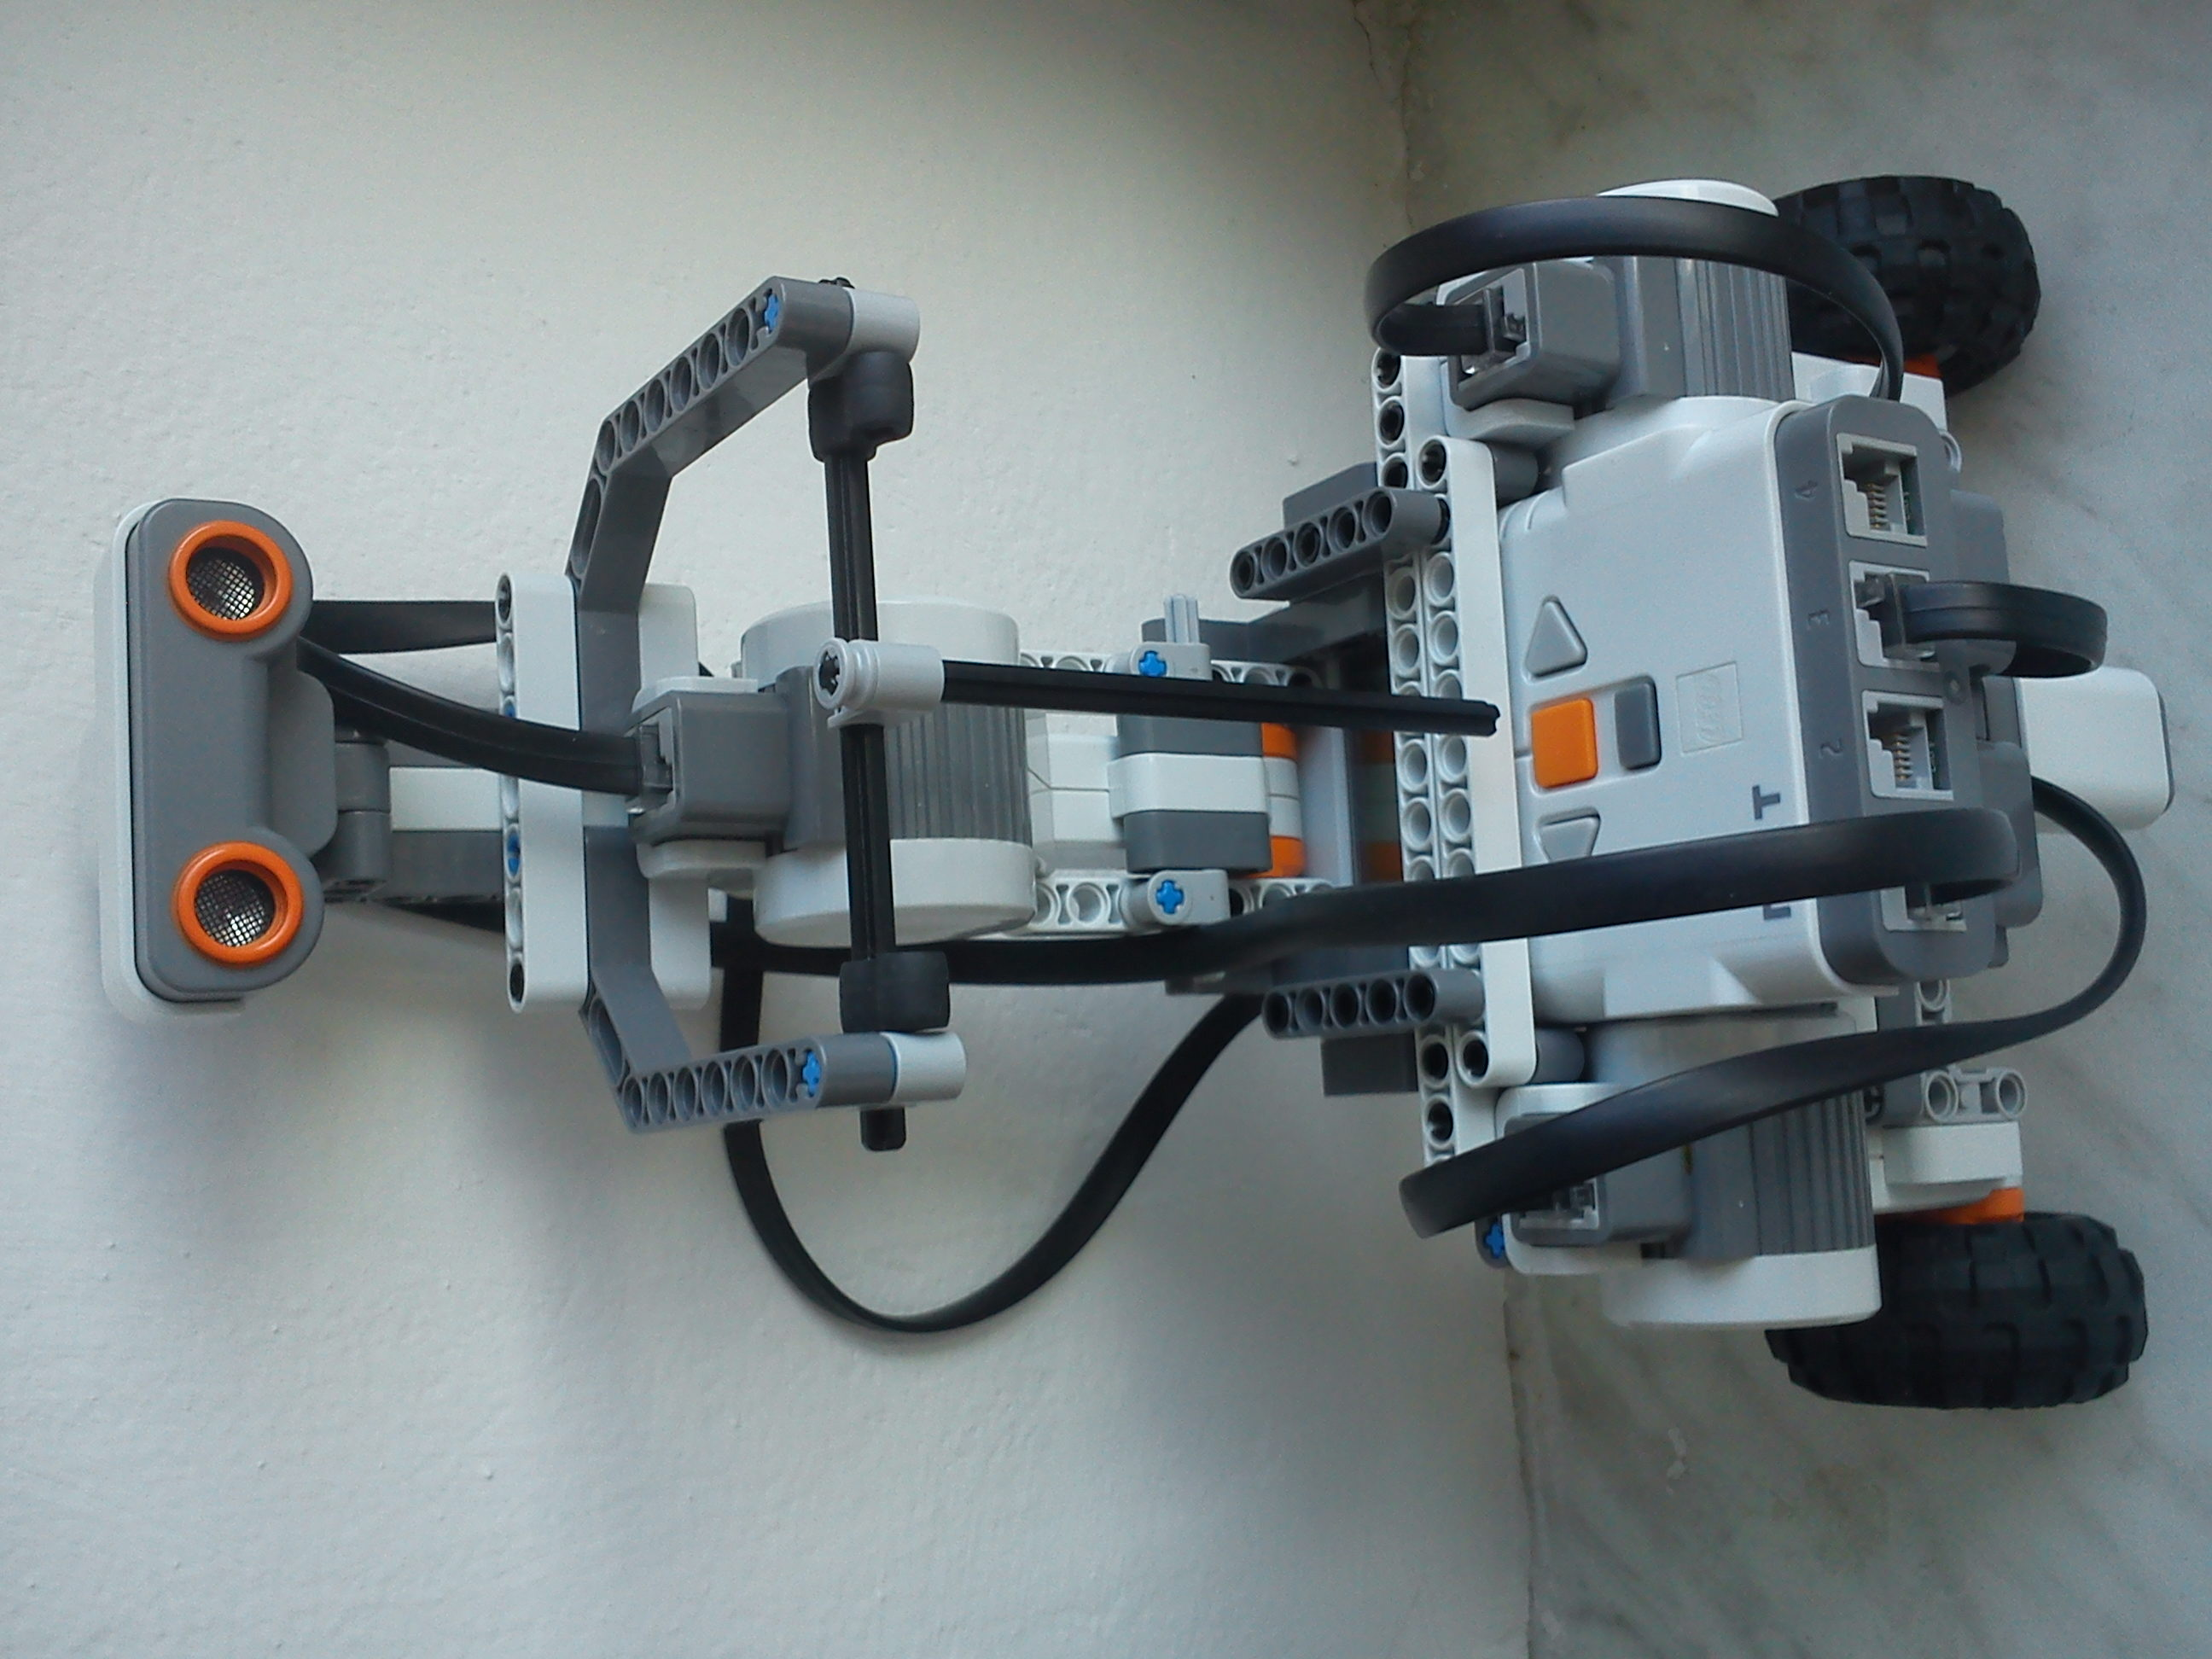
\includegraphics[width=7cm, angle=270]{legway}
    \caption{Legway}
    \label{fig:legway}
\end{figure}

The communication with Lego brick is done over bluetooth. Initially we intended
to use ultrasonic sensor to avoid obstacles but later we decided to remove
unnecessary parts to lower the centre of gravity to solve our problems with
balancing.

For different parts of the project our team used different programming
languages. The main program of the robot is written in NXC \cite{nxc} which is a
language very similar to C. Testing module for bluetooth communication is
written in Ruby and finally the application for controlling the segway is
written in Scala.

Unfortunately during our work on this project we experienced display failure on
Lego brick two times. This caused delay in our work and the second malfunction
prevented us from merging the codebases of team members and from enough
experimentation with controller parameters as our team used the display for
debugging purposes.

\section{Controller}

\section{Bluetooth}

\section{Scheduling}

\section{Conclusion}

\printbibliography

\end{document}
